\documentclass[10pt,twocolumn,letterpaper]{article}

\usepackage{cvpr}
\usepackage{times}
\usepackage{epsfig}
\usepackage{graphicx}
\usepackage{amsmath}
\usepackage{amssymb}

% Include other packages here, before hyperref.

% If you comment hyperref and then uncomment it, you should delete
% egpaper.aux before re-running latex.  (Or just hit 'q' on the first latex
% run, let it finish, and you should be clear).
\usepackage[breaklinks=true,bookmarks=false]{hyperref}

\cvprfinalcopy % *** Uncomment this line for the final submission

\def\cvprPaperID{****} % *** Enter the CVPR Paper ID here
\def\httilde{\mbox{\tt\raisebox{-.5ex}{\symbol{126}}}}

% Pages are numbered in submission mode, and unnumbered in camera-ready
%\ifcvprfinal\pagestyle{empty}\fi
\setcounter{page}{1}
\begin{document}

%%%%%%%%% TITLE
\title{Yelp Recommendations}

\author{
Gavriel Adler\\
Carnegie Mellon University\\
{\tt\small gya@andrew.cmu.edu}
% For a paper whose authors are all at the same institution,
% omit the following lines up until the closing ``''.
% Additional authors and addresses can be added with ``\and'',
% just like the second author.
% To save space, use either the email address or home page, not both
\and
Spencer Barton\\
Carnegie Mellon University\\
{\tt\small sebarton@andrew.cmu.edu}
\and
Fridtjof Melle\\
Carnegie Mellon University\\
{\tt\small fmelle@andrew.cmu.edu}
}

\maketitle
%\thispagestyle{empty}

%%%%%%%%% ABSTRACT
\begin{abstract}
   When looking for somewhere to eat, people often read online reviews of restaurants they have not visited themselves. One of the most common websites that aggregates user reviews is \url{http://www.yelp.com}. Using machine learning techniques, we aimed make this process simpler by giving users specific restaurant recommendations, replacing their time spent looking through many possible places to eat, turning down many or most of them, with a small subset of restaurants the user is likely to enjoy based on the reviews of similar users.

   
\end{abstract}

%%%%%%%%% BODY TEXT
\section{Introduction}

\subsection{The Problem}
\url{http://www.yelp.com} is a popular destination for people looking to find out what other people think of restaurants, coffee shops, and other food establishments in their area. Often people make decisions on where to eat based on the reviews other yelp members give to restaurants they're considering. While this is more useful than having no information about the restaurant at all, someone looking for a recommendation is bound to the opinions of strangers, who perhaps have very different tastes in food. 
\subsection{The Solution}
Our solution is to fix this problem by giving a person personalized recommendations. Based on the person's past reviews, we aim to find a subset of \textit{Yelp} users with similar taste and guess the scores that the given person would give to restaurants he or she has not yet visited. This allows the person to try a new restaurant with a greater sense of security that he or she will enjoy the experience and not waste money. \cite{Alpher02}

\section{Data Set}
\subsection{Overview}
\textit{Yelp} holds a massive amount of data to their disposal based on everything that users provide in terms of personal information, business information and everything they put into their reviews. For our purpose \textit{Yelp} provides a subset of this based on a specific region or city, generated with the same attributes as the real world data, which for our case is Phoeniz, AZ. This provides us with a total of 14303 restaurants and 1.2M reviews, all connected to Phoeniz through around 250000 users.

\subsection{Users}
In order to generate a user characterizing model we were inclined to extract all the elite users as they contain the most data and will be the easiest to map for interests and taste. These users count a total of 20045 individuals, all with an average of 200 reviews each. This gives us a good basis to develop a model. In addition we have randomly extracted 2014 sample users not contained within the training data, to test our algorithm on, as well as the top 50 reviewers from the elite users to test the pipeline on. All users are in the same reduced format, only containing the parameters we deem necessary for characterizing the particular users. Removed attributes primarily include \textit{friends}. The data is originally compiled in JSON, which we have expanded to operate on, and then convert to CSV for classification and prediction.

\begin{verbatim}
	{
        "average_stars": 3.65,
        "compliments": {
            "cool": 16,
            "funny": 5,
            "hot": 8,
            "more": 1,
            "note": 3,
            "plain": 9,
            "profile": 1,
            "writer": 4
        },
        "elite": [
            2013,
            2014
        ],
        "fans": 7,
        "name": "Lene",
        "review_count": 214,
        "user_id": "WvhiRlcyEiy-XYwiCofzdg",
        "votes": {
            "cool": 110,
            "funny": 56,
            "useful": 274
        },
        "yelping_since": "2010-10"
    }
\end{verbatim}

\subsection{Restaurants}


\subsection{Reviews}

\section{Algorithm Overivew}
\subsection{The Pipeline}
\begin{figure}[t]
\begin{center}
\fbox{\rule{0pt}{2in}
   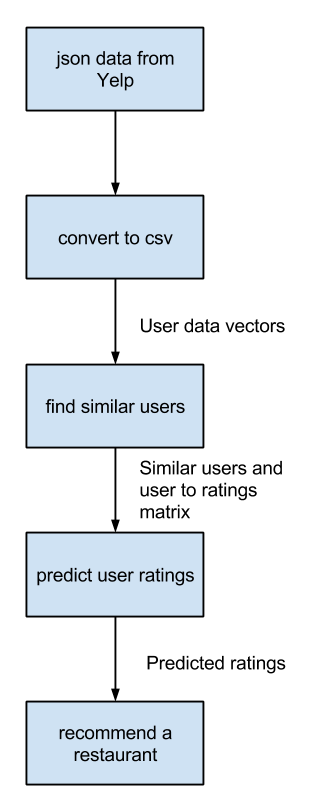
\includegraphics[width=0.8\linewidth]{WorkFlow.png}}
\end{center}
   \caption{A workflow diagram of our pipeline.}
\label{fig:long}
\label{fig:onecol}
\end{figure}

Our pipeline takes in a person, and outputs a restaurant recommendation. In order to do this we first create a feature vector for the person, and find a list of similar users based on these features. We then see how these similar users rated restaurants the person has not been to, and therefore guess how the person would rate those restaurants. Finally, the restaurants with the highest expected ratings are returned to the user.
\subsection{Similar Users and Restaurant Rating Prediction}
Our solution creates a feature vector of each user and uses the Kth Nearest Neighbor algorithm to cluster the feature vectors and find K users closest to the person based on the feature vector. We then take a weighted average of the reviews from those users for every restaurant the person has not visited to guess how that person would rate those restaurants.

\section{What We Have Done}
\subsection{Parsing the Data}
The \textit{Yelp} dataset is very large, and so we have parsed it down and removed a small subset to work with. We took the data for the top 50 users, and all the restaurants they have visited, as well as their reviews of them, and the personal data \textit{Yelp} stores for those users. We converted all the data from JSON objects to easy to load and work with .csv files. The scripts which do this can easily be changed to load in data for a different set of users and save the same .csv files.
\subsection{Making User Vectors and Finding Similar Users}
Right now our user vectors are based on the user's \textit{Yelp} profiles. Yelp user reviews can be rated by other users as "funny", "useful", and "cool". Users can also compliment other users in many ways. We vectorize all of a users ratings and complements, as well as append the user \textit{Yelp} statistics (fans, average review, and number of reviews). This feature vector gives us an idea of how other users view this user in the \textit{Yelp} community. This feature vector was a quick way to create a feature vector that we could use and test in our pipeline, in the future we plan to add food and restaurant-specific features. To find similar usres, we simply run KNN for a single user feature vector on the entire set of user feature vectors. Modifying the feature vector is one of the key steps we plan to work on in the next half of the project.
\subsection{Guessing User Reviews}
Right now, to guess a user review, we take two things into account: the ratings a user's similar users rated a restaurant and the average rating of the restaurant overall We weight each by a half to guess how a user would rate a restaurant.
\subsection{Implementation}
Our code is implemented in Python's PANDAS module. Coding in Python allows us to rapidly prototype and get things working in the short amount of time we have to do the project. PANDAS, being strictly typed and implemented in C, speeds of computation time considerably and allows us to run our code on a much larger dataset. The code is visible at \url{https://github.com/sbarton272/PatRec}.

\section{What We Plan to Do}

\section{Issues and Potential Issues}

%uncomment and add \cite{}'s for bilbiography. fill in egbib.bib file
{\small
\bibliographystyle{ieee}
\bibliography{egbib}}


\end{document}
